\documentclass{beamer}
\usepackage[utf8]{inputenc}
\usepackage{xeCJK} 
\usepackage[T1]{fontenc}
\usepackage{mathabx}
\usepackage{amsmath} 
\usepackage{mathpazo}
\usepackage{bibentry}
\usepackage{tikz}
\usepackage{caption}
\usepackage{graphicx}
\usepackage{subfigure}
\usepackage{animate}
\usepackage{hyperref}

\usetikzlibrary{scopes}
\def\iangle{35} % Angle of the inclined plane
\def\down{-90}
\def\arcr{0.5cm} % Radius of the arc used to indicate angles

\usetheme{Boadilla}
\usecolortheme{wolverine}
\useoutertheme{miniframes}

\title{VP160 Recitation Class VIII}
\subtitle{Statics}
\author{Zeyi Ren}
\institute{UM-SJTU Joint Institute}

\begin{document}

\maketitle

\frame{\tableofcontents}

\section{Statics of Rigid Body}
\begin{frame}{Equilibrium}
  \begin{block}{Equilibrium}
    %The sum of all the external forces is equal to zero
    $$F_{ext} = 0$$
    %The sum of all torques of external forces about any point is equal to zero
    $$\tau_{ext} = 0$$
  \end{block}\pause
  \begin{itemize}
    \item The sum of all the external forces is equal to zero\pause
    \item The sum of all torques of external forces about any point is equal to zero
  \end{itemize}\pause
  $$\Rightarrow \text{If the object is initially at rest, then it will remain at rest.}$$
\end{frame}

\begin{frame}{Center of Gravity}
  \begin{block}{Center of Gravity}
    A point from which the weight of a body or system may be considered to act. In uniform gravity it is the same as the center of mass.
  \end{block}\pause
  \begin{itemize}
    \item For translational motion: $$\vec{G} = M\vec{a_c}$$\pause
    \item For rotation: $$\vec{\tau_{tot}} = \sum \vec{r_i}\times \vec{G_i}$$\pause
    If in a uniform gravitaional field (mostly):
    $$\vec{\tau_{tot}}= \sum m_i\vec{r_i}\times \vec{g} = M\frac{\sum m_i\vec{r_i}}{\sum m_i}\times \vec{g} = M\vec{r_c}\times \vec{g} = \vec{r_c}\times \vec{G}$$
  \end{itemize}
\end{frame}

\begin{frame}{Methods for Solving Statics}
  \begin{enumerate}
    \item Equilibrium equations. \pause
    \begin{itemize}
      \item Translational motion: Force \pause
      \item Rotation: Torque\pause
    \end{itemize}
    \item Virtual work\pause
    \begin{itemize}
      \item \textbf{Principle of Virtual Work}\pause
      %: \\If a particle(or system, or rigid body) is in equilibrium, the total virtual work of forces acting on the object is zero for any virtual displacement.
    \end{itemize}
    \item Infinitesimal methods\pause
    \item Derivation of energy\pause
    \begin{itemize}
      \item $\frac{\partial U}{\partial q_i} = 0$, the system potential energy reaches an local minimum.\pause
      \item useful for low degree of freedom system.
    \end{itemize}
  \end{enumerate}
\end{frame}

\begin{frame}{Equilibrium equations \& Infinitesimal methods}
\textcolor{blue}{Exercise 1}

Find the tension force inside the strain, as shown in the figure below. $m$ and $\alpha$ are known.
\begin{figure}[htbp]
\centering
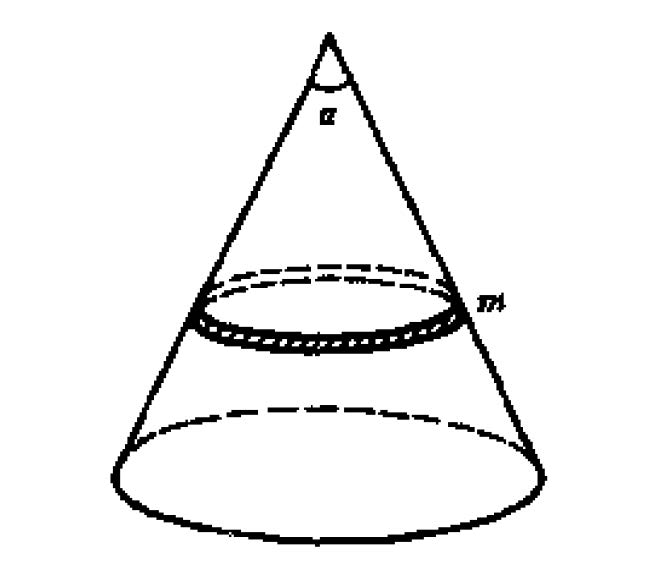
\includegraphics[width=0.4 \linewidth, angle =0]{ex1.png}
%\caption{.}
\label{fig:1}
\end{figure}
\end{frame}

\begin{frame}{Virtual Work}
\textcolor{blue}{Exercise 2}

A half cylinder is placed on the horizontal plane, and is covered by a uniform chain with length $\pi r$ and linear density $\lambda$. Find the tensile force of the chain at the top of the cylinder.
\begin{figure}[htbp]
\centering
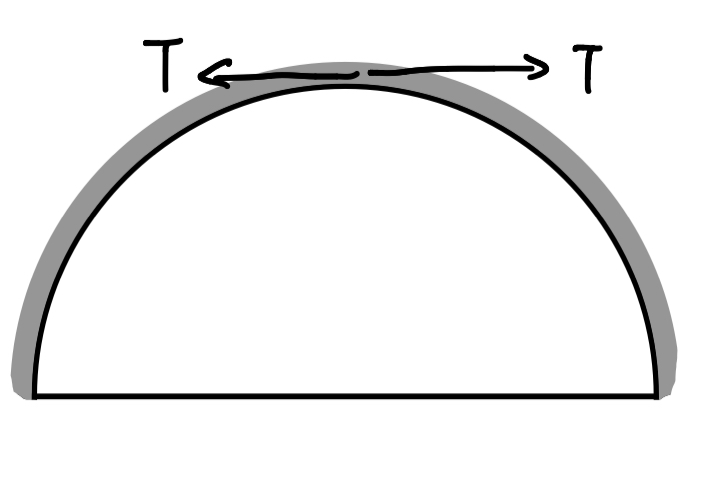
\includegraphics[width=0.4 \linewidth, angle =0]{ex2.png}
%\caption{.}
\label{fig:2}
\end{figure}
\end{frame}

\begin{frame}{Extended materials on virtual work (for your interest)}
 \begin{figure}[htbp]
 \centering
 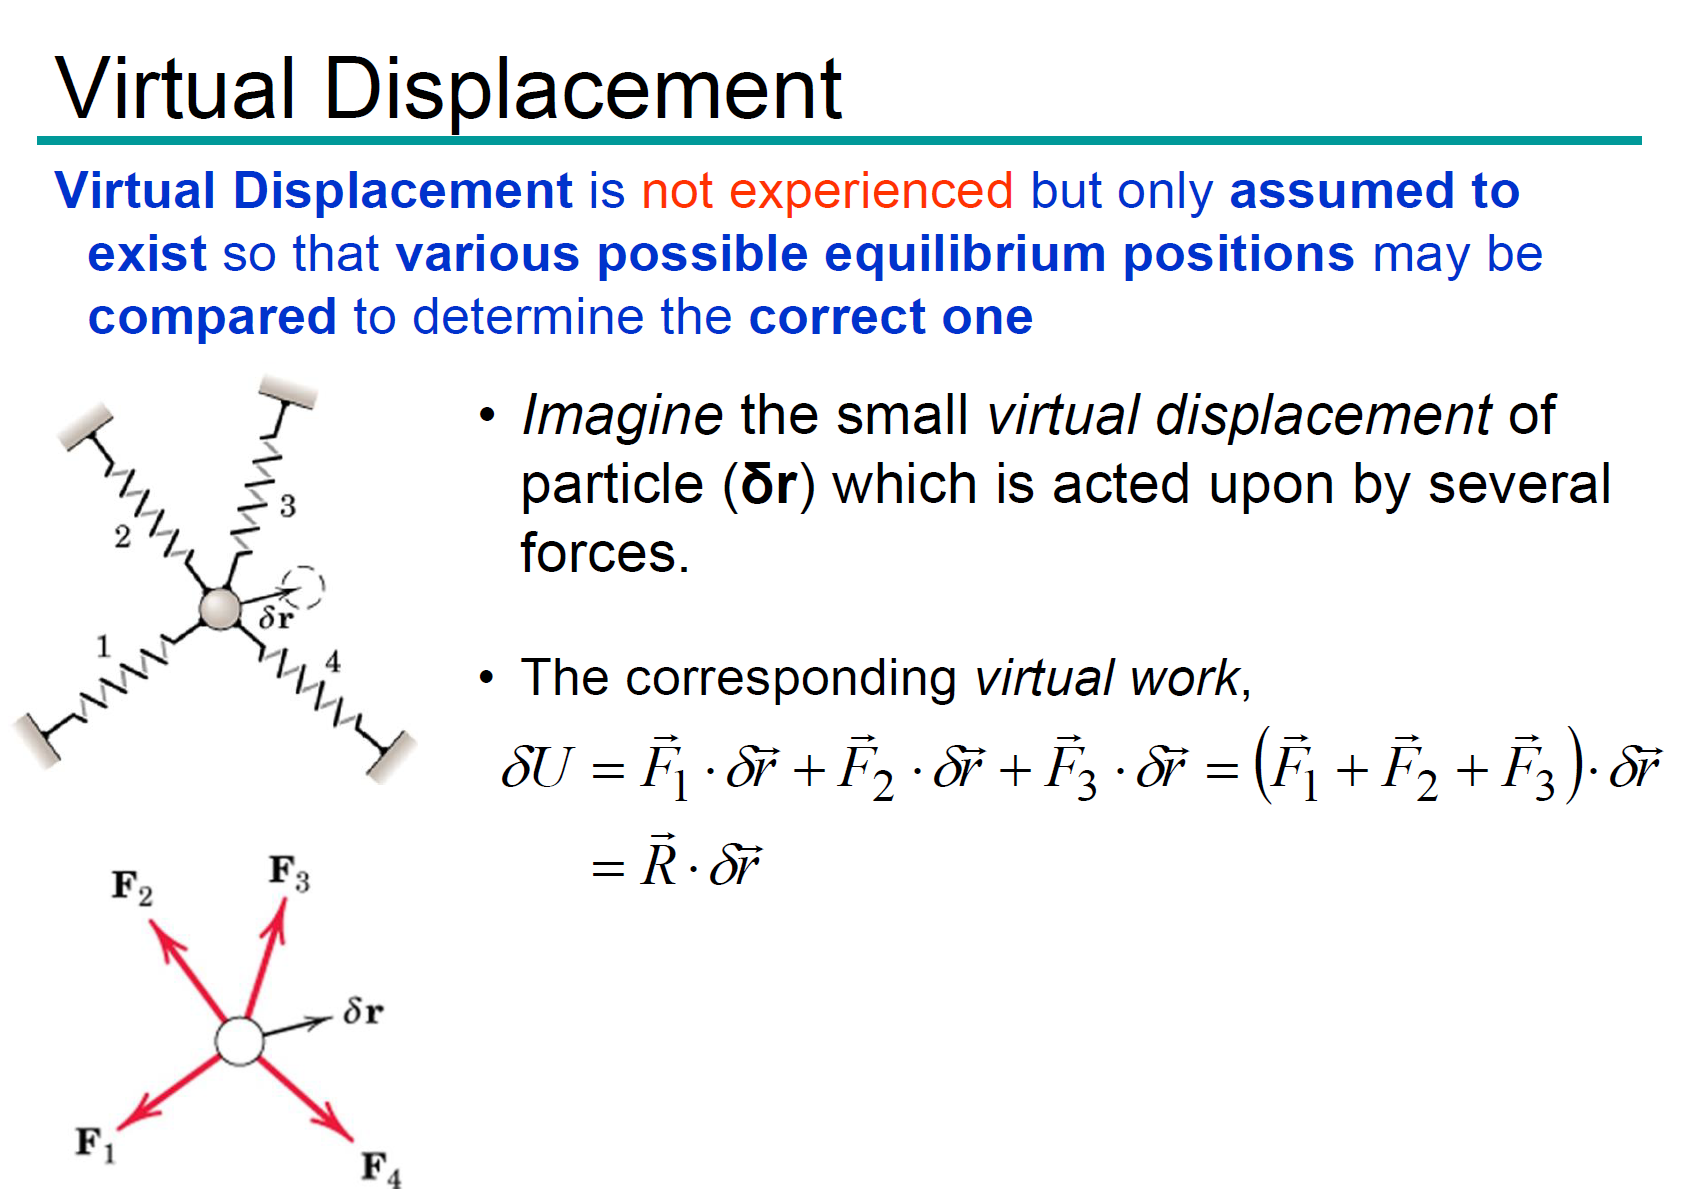
\includegraphics[width=0.8 \linewidth, angle =0]{virtual_work1.png}
 %\caption{.}
 \label{fig:v1}
 \end{figure}
\end{frame}

\begin{frame}
  \begin{figure}[htbp]
  \centering
  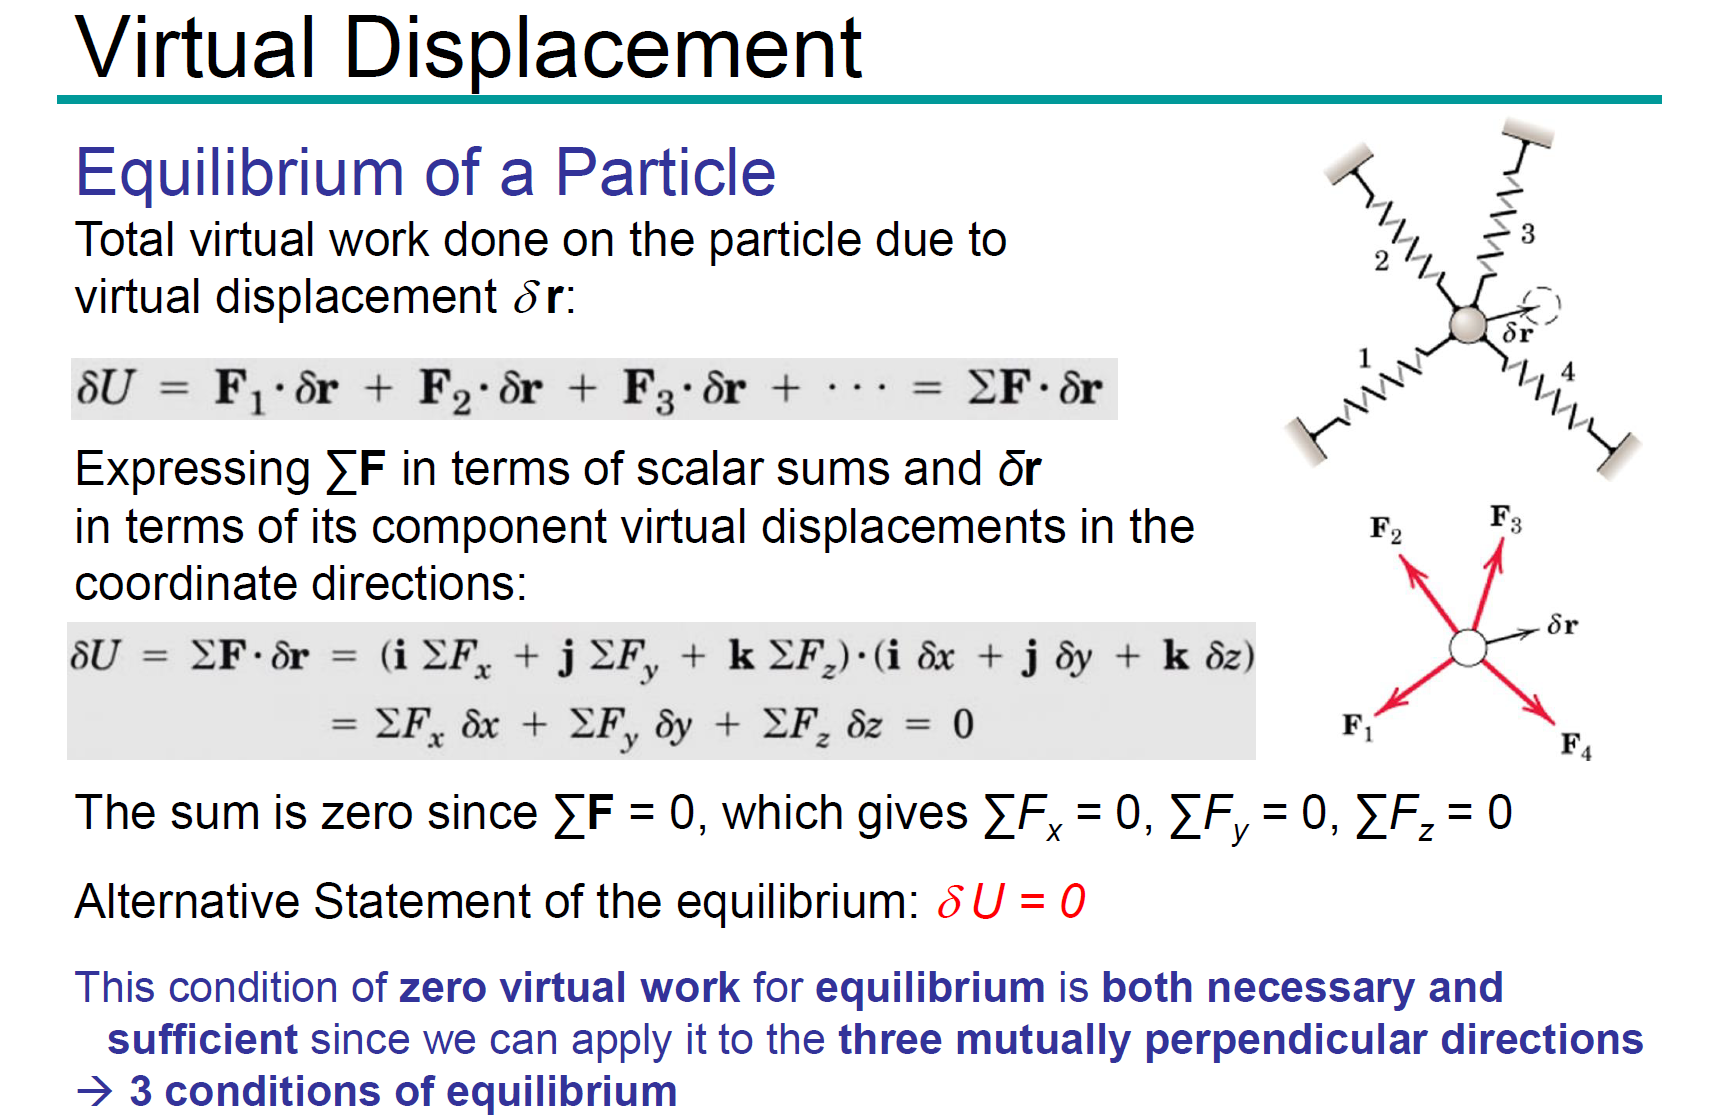
\includegraphics[width=1 \linewidth, angle =0]{virtual_work2.png}
  %\caption{.}
  \label{fig:v2}
  \end{figure}
\end{frame}

\begin{frame}
  \begin{figure}[htbp]
  \centering
  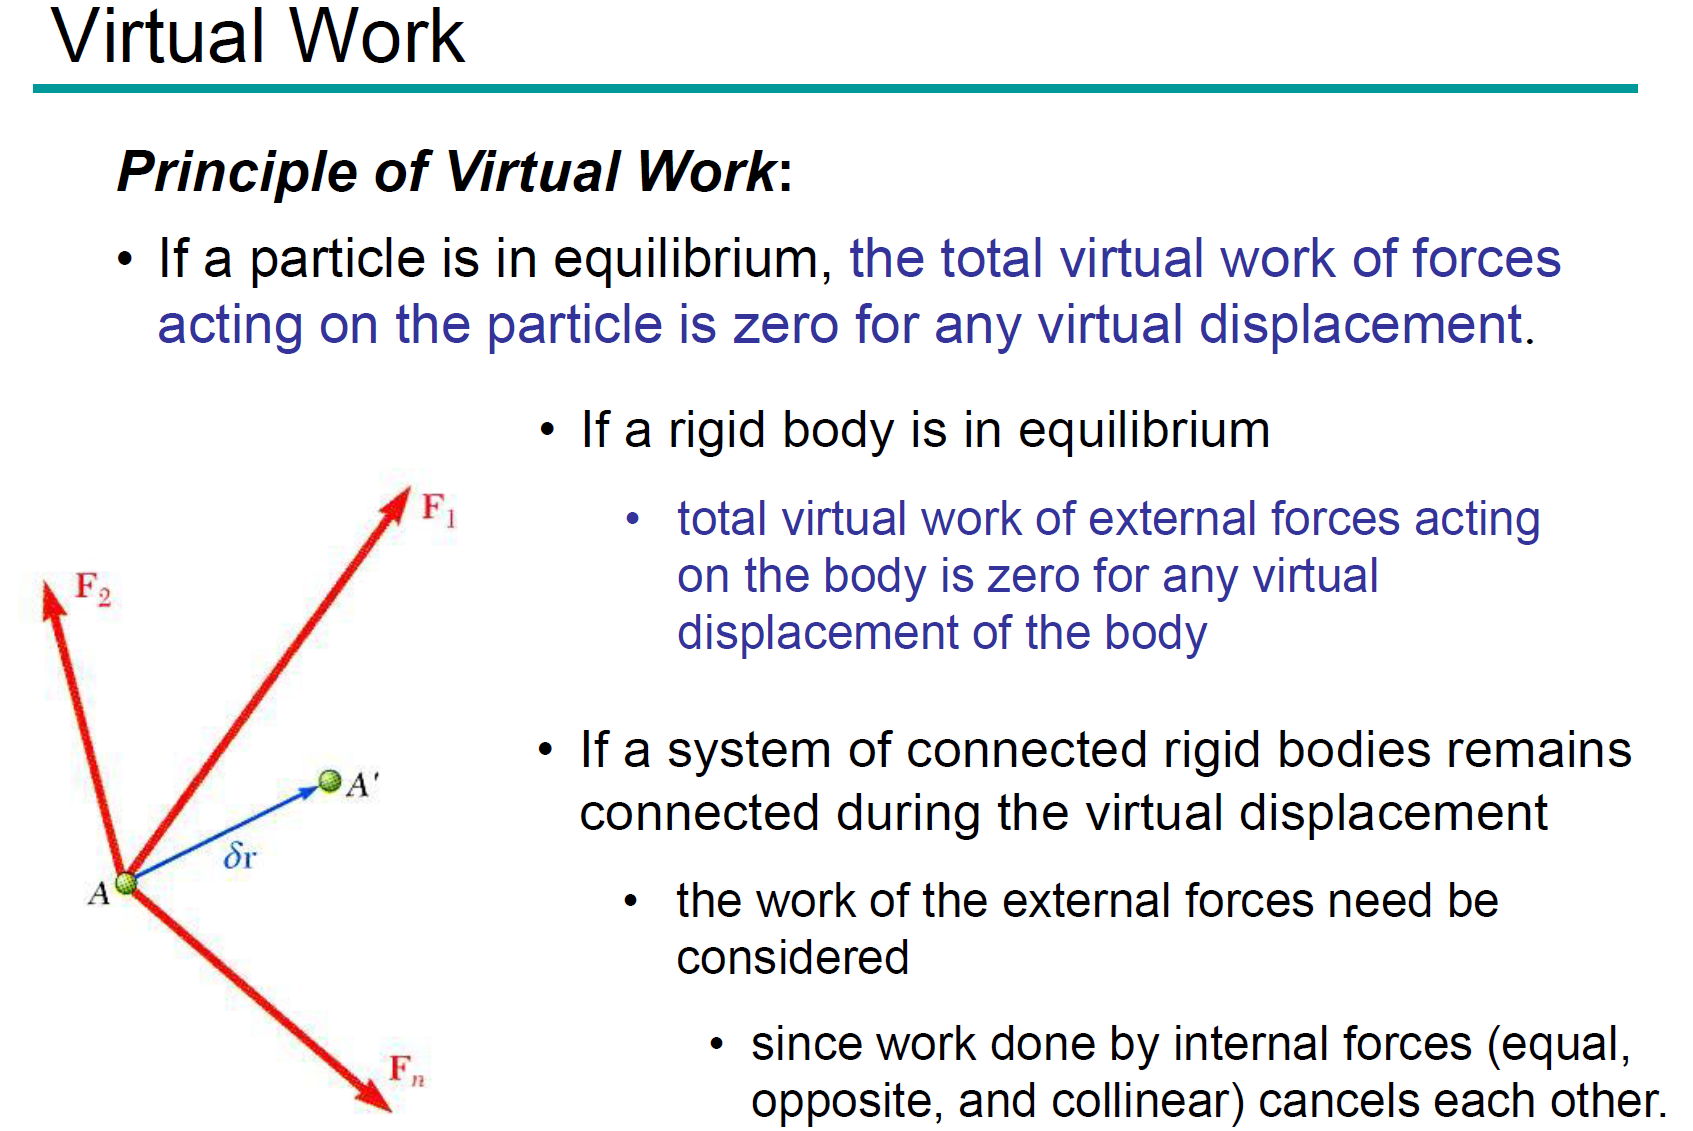
\includegraphics[width=0.9 \linewidth, angle =0]{virtual_work3.png}
  %\caption{.}
  \label{fig:v3}
  \end{figure}
\end{frame}

\begin{frame}{Equilibrium equations}
\textcolor{blue}{Exercise 3}

Three cylinders have same mass and radius. Friction coefficient between two cylinders is $\mu_1$, between cylinder and ground is $\mu_2$.
Find the minimum of $\mu_1$ and $\mu_2$ respectively, so that the system is in static.
\begin{figure}[htbp]
\centering
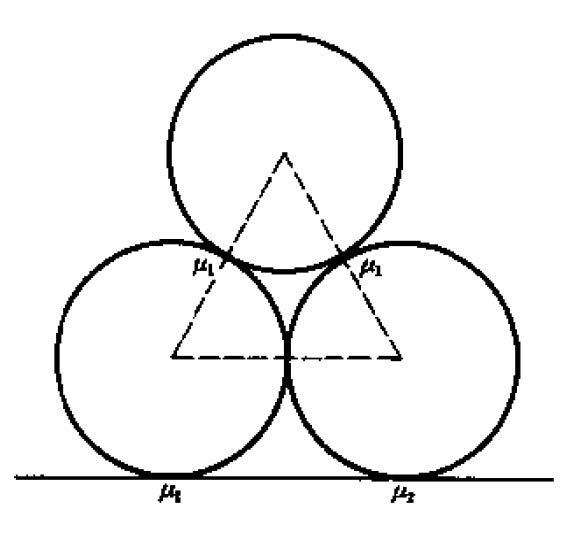
\includegraphics[width=0.4 \linewidth, angle =0]{ex3.png}
%\caption{.}
\label{fig:3}
\end{figure}
\end{frame}

\begin{frame}{Derivation of energy}
\textcolor{blue}{Exercise 4}

Find $\theta$ when the system is in static. Assume $l = 50cm$, $m = 50g$, $r = 8cm$, $M = 200g$.
\begin{figure}[htbp]
\centering
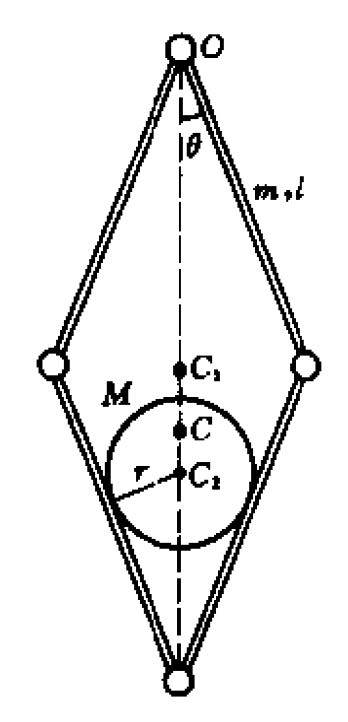
\includegraphics[width=0.2 \linewidth, angle =0]{ex4.png}
%\caption{.}
\label{fig:4}
\end{figure}
\end{frame}

\section{Elasticity}
\begin{frame}
  \begin{block}{Stress}
    Stress is the force per unit area.
  \end{block}\pause
  \begin{block}{Strain}
    Strain is the fractional deformation due to the stress.
  \end{block}\pause
  $$\text{elastic modulus } = \frac{\text{stress}}{\text{strain}}$$
\end{frame}

\begin{frame}
  \begin{block}{Young's modulus: tensile stress divided by tensile strain}
    $$Y = \frac{\frac{F\bot }{A}}{\frac{\Delta l}{L}}$$
  \end{block}\pause
  \begin{figure}[htbp]
  \centering
  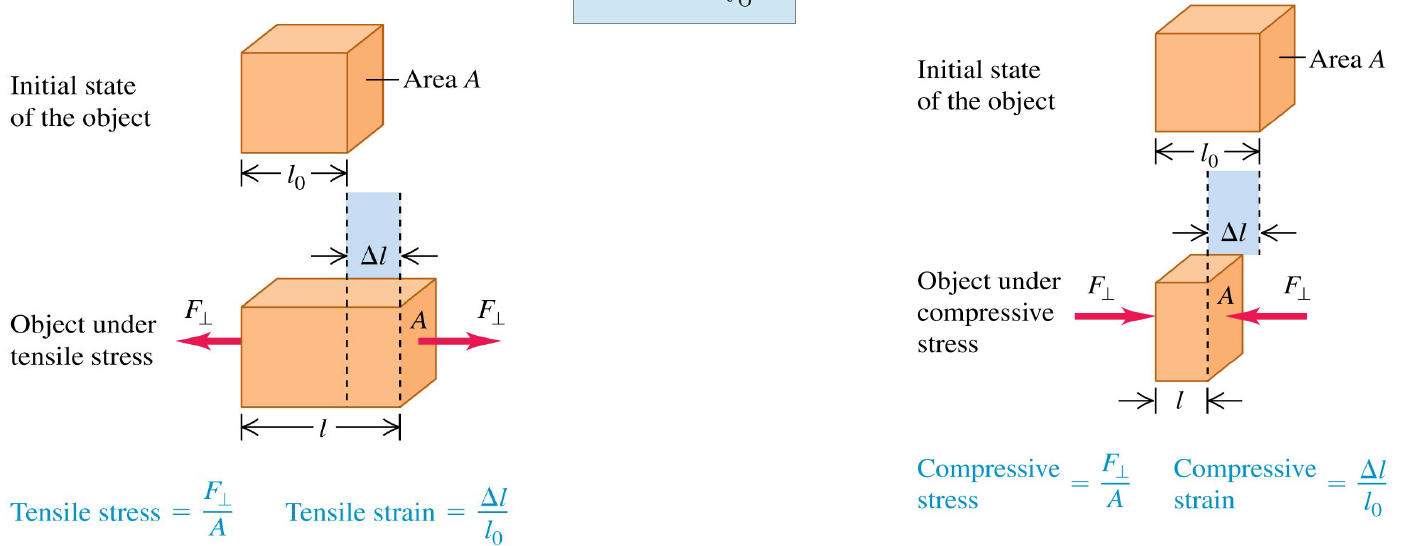
\includegraphics[width=1 \linewidth, angle =0]{y's.png}
  %\caption{.}
  \label{fig:y's}
  \end{figure}
\end{frame}

\begin{frame}
  \begin{block}{Bulk's modulus: bulk stress divided by bulk strain}
    $$B=-\frac{\Delta p}{\frac{\Delta v}{V}}$$
  \end{block}\pause
  \begin{figure}[htbp]
  \centering
  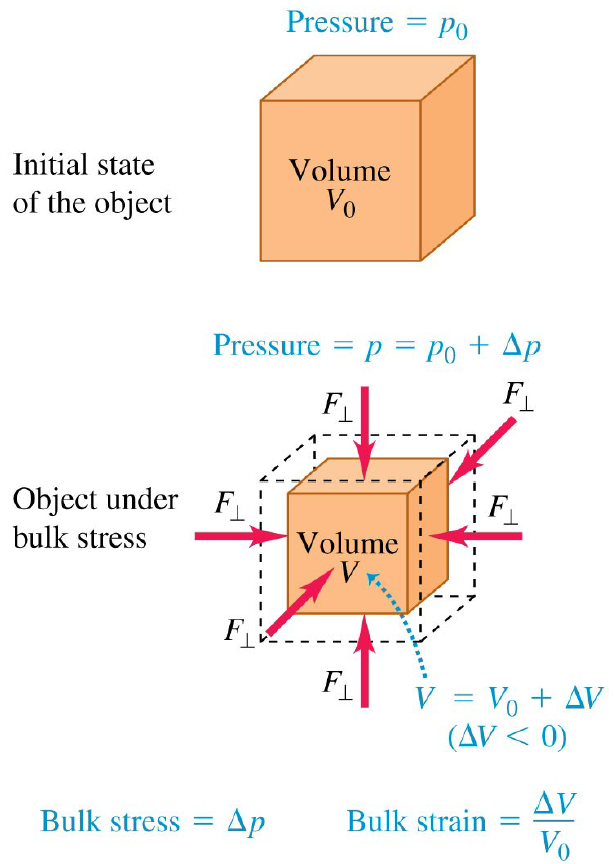
\includegraphics[width=0.4 \linewidth, angle =0]{b's.png}
  %\caption{.}
  \label{fig:b's}
  \end{figure}
\end{frame}

\begin{frame}
  \begin{block}{Shear modulus: shear stress divided by shear strain}
    $$S=\frac{\frac{F_{\|}}{A}}{\frac{X}{h}}$$
  \end{block}\pause
  \begin{figure}[htbp]
  \centering
  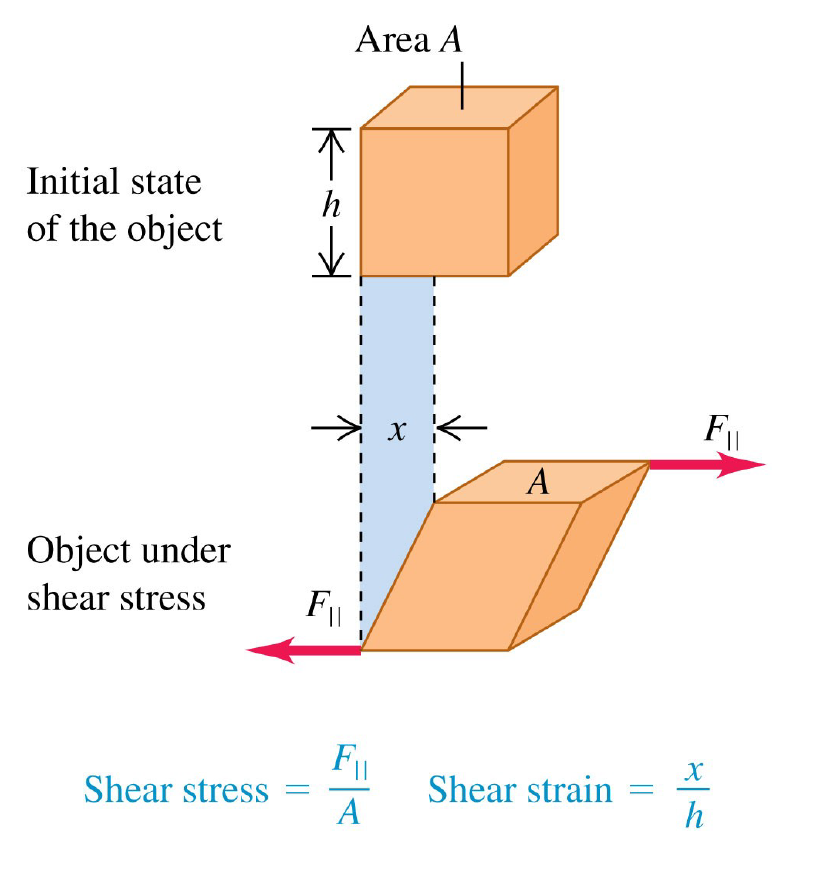
\includegraphics[width=0.4 \linewidth, angle =0]{s's.png}
  %\caption{.}
  \label{fig:s's}
  \end{figure} 
\end{frame}

\begin{frame}{Write at the end}
  \begin{itemize}
    \item The remaining part will be covered in the final recitaion class (they are relatively simple).\pause
    \item You are almost done! Thanks for your hard-working!\pause
    \item I really want to continue to be your VP260 TA, but may not be able to...keep in touch, I'm willing to help, not only in Physics. \pause
    \item Wish you all the best in your future life and find your own way in JI!\pause
  \end{itemize}
  \centering
  \LARGE{Thanks!}
\end{frame}

\begin{frame}{Reference}
  \begin{thebibliography}{9}
  \setbeamertemplate{bibliography item}[article]
  \bibitem{C} Yigao Fang.\\
  \textcolor{black}{VP160 Recitation Slides.}\\
  2020
  \bibitem{C} Haoyang Zhang.\\
  \textcolor{black}{VP160 Recitation Slides.}\\
  2020
  \setbeamertemplate{bibliography item}[book]
  \bibitem{C} Yousheng Shu (舒幼生).\\
  \textcolor{black}{\textit{Mechanics (力学)}}\\
  Peking University Press, 2005
  % \setbeamertemplate{bibliography item}[book]
  % \bibitem{C} Jiafu Cheng (程稼夫).\\
  % \textcolor{black}{\textit{中学奥林匹克竞赛物理教程:力学篇}}\\
  % University of Science and Technology Press, 2013
  \end{thebibliography}
  \end{frame}
  \end{document}



